% !Mode:: "TeX:UTF-8:Main"
% gif command (hope it still works ...)
% magick -density 160 -delay 35 -loop 0 XXXX.pdf XXXX.gif

\documentclass{beamer}
\usepackage[T1]{fontenc} % or fontspec if lualatex is wanted ...
\setbeamertemplate{navigation symbols}{}
\usepackage{tikzducks,tikzlings,bearwear}
\usetikzlibrary{calc}
\usepackage{bearwear}
\begin{document}

\begin{frame}

\begin{tikzpicture}[remember picture,overlay]
	
% Background image
\node[at=(current page.center)]{%
	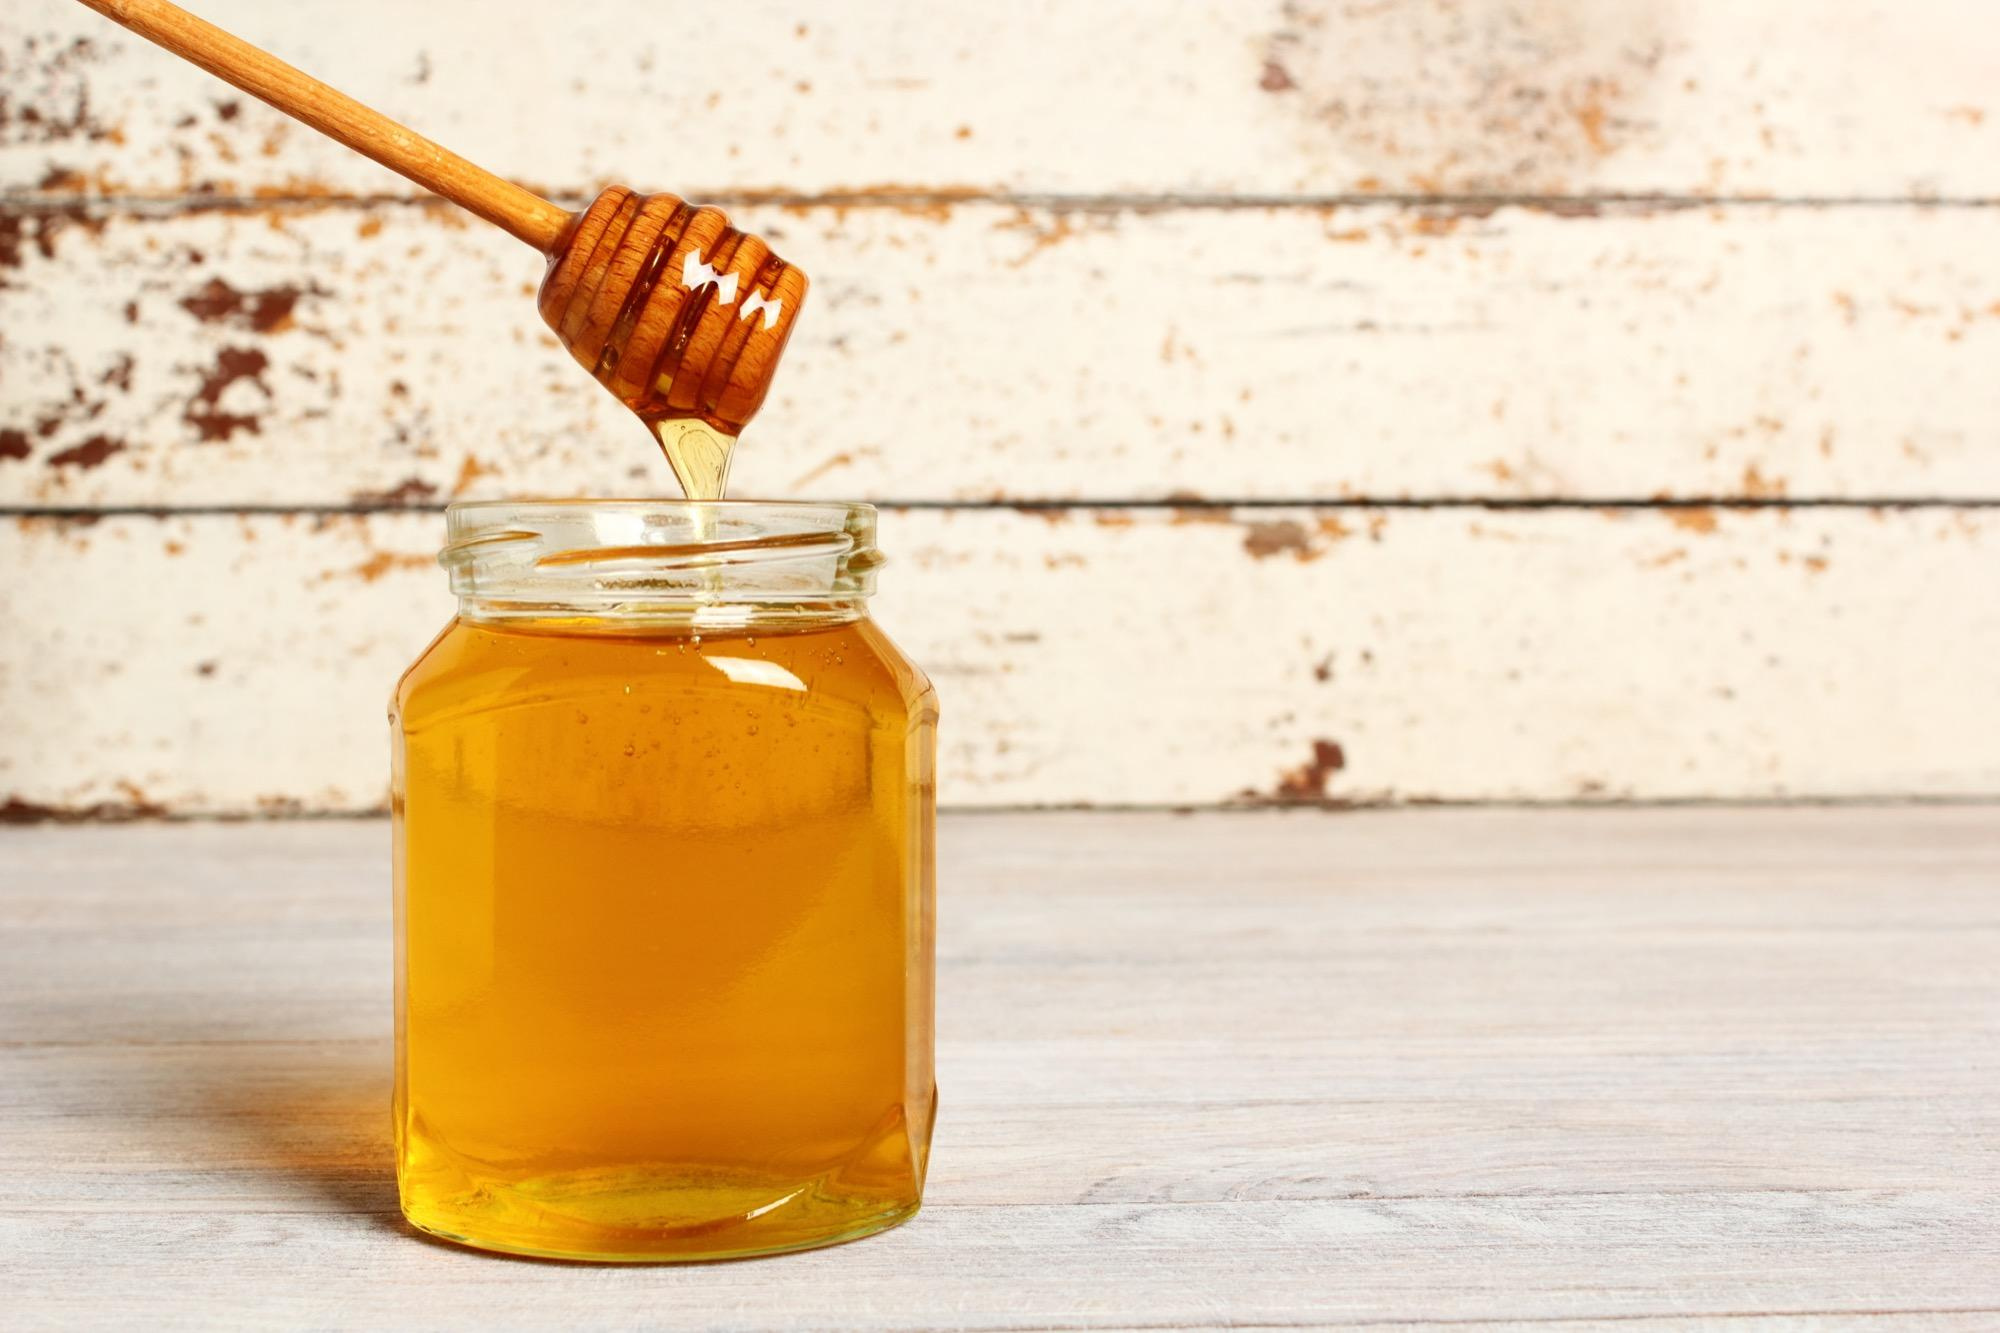
\includegraphics[height=1.05\paperheight]{honey-pot}%%% later
};	
% Image credit of background

\foreach \X [evaluate=\X as \Y using {sin(\X)}]in %{0,1}
{0,5,...,3500}
{
  \only<+>{%
    \begin{scope}[scale=2,shift={($(current page.south)+(1,1+0.8*\Y)$)}]
    \bear\bearwear[shirt=white,
     body deco={
     \node[] at ([yshift=-0.3mm]beartummy){%
      
\includegraphics[scale=0.6]{michelinstern-crop}%
      
\includegraphics[scale=0.6]{michelinstern-crop}%
      
\includegraphics[scale=0.6]{michelinstern-crop}};
      }]
    \node[] at ([yshift=2.5mm,xshift=0.9cm]beartummy) {
\includegraphics[trim=0cm 0cm 0.7cm 0cm,clip,width=2cm,angle=20]{spoon}};
    \end{scope}
}}
\end{tikzpicture}
\end{frame}
\end{document}
